\documentclass[1p]{elsarticle_modified}
%\bibliographystyle{elsarticle-num}

%\usepackage[colorlinks]{hyperref}
%\usepackage{abbrmath_seonhwa} %\Abb, \Ascr, \Acal ,\Abf, \Afrak
\usepackage{amsfonts}
\usepackage{amssymb}
\usepackage{amsmath}
\usepackage{amsthm}
\usepackage{scalefnt}
\usepackage{amsbsy}
\usepackage{kotex}
\usepackage{caption}
\usepackage{subfig}
\usepackage{color}
\usepackage{graphicx}
\usepackage{xcolor} %% white, black, red, green, blue, cyan, magenta, yellow
\usepackage{float}
\usepackage{setspace}
\usepackage{hyperref}

\usepackage{tikz}
\usetikzlibrary{arrows}

\usepackage{multirow}
\usepackage{array} % fixed length table
\usepackage{hhline}

%%%%%%%%%%%%%%%%%%%%%
\makeatletter
\renewcommand*\env@matrix[1][\arraystretch]{%
	\edef\arraystretch{#1}%
	\hskip -\arraycolsep
	\let\@ifnextchar\new@ifnextchar
	\array{*\c@MaxMatrixCols c}}
\makeatother %https://tex.stackexchange.com/questions/14071/how-can-i-increase-the-line-spacing-in-a-matrix
%%%%%%%%%%%%%%%

\usepackage[normalem]{ulem}

\newcommand{\msout}[1]{\ifmmode\text{\sout{\ensuremath{#1}}}\else\sout{#1}\fi}
%SOURCE: \msout is \stkout macro in https://tex.stackexchange.com/questions/20609/strikeout-in-math-mode

\newcommand{\cancel}[1]{
	\ifmmode
	{\color{red}\msout{#1}}
	\else
	{\color{red}\sout{#1}}
	\fi
}

\newcommand{\add}[1]{
	{\color{blue}\uwave{#1}}
}

\newcommand{\replace}[2]{
	\ifmmode
	{\color{red}\msout{#1}}{\color{blue}\uwave{#2}}
	\else
	{\color{red}\sout{#1}}{\color{blue}\uwave{#2}}
	\fi
}

\newcommand{\Sol}{\mathcal{S}} %segment
\newcommand{\D}{D} %diagram
\newcommand{\A}{\mathcal{A}} %arc


%%%%%%%%%%%%%%%%%%%%%%%%%%%%%5 test

\def\sl{\operatorname{\textup{SL}}(2,\Cbb)}
\def\psl{\operatorname{\textup{PSL}}(2,\Cbb)}
\def\quan{\mkern 1mu \triangleright \mkern 1mu}

\theoremstyle{definition}
\newtheorem{thm}{Theorem}[section]
\newtheorem{prop}[thm]{Proposition}
\newtheorem{lem}[thm]{Lemma}
\newtheorem{ques}[thm]{Question}
\newtheorem{cor}[thm]{Corollary}
\newtheorem{defn}[thm]{Definition}
\newtheorem{exam}[thm]{Example}
\newtheorem{rmk}[thm]{Remark}
\newtheorem{alg}[thm]{Algorithm}

\newcommand{\I}{\sqrt{-1}}
\begin{document}

%\begin{frontmatter}
%
%\title{Boundary parabolic representations of knots up to 8 crossings}
%
%%% Group authors per affiliation:
%\author{Yunhi Cho} 
%\address{Department of Mathematics, University of Seoul, Seoul, Korea}
%\ead{yhcho@uos.ac.kr}
%
%
%\author{Seonhwa Kim} %\fnref{s_kim}}
%\address{Center for Geometry and Physics, Institute for Basic Science, Pohang, 37673, Korea}
%\ead{ryeona17@ibs.re.kr}
%
%\author{Hyuk Kim}
%\address{Department of Mathematical Sciences, Seoul National University, Seoul 08826, Korea}
%\ead{hyukkim@snu.ac.kr}
%
%\author{Seokbeom Yoon}
%\address{Department of Mathematical Sciences, Seoul National University, Seoul, 08826,  Korea}
%\ead{sbyoon15@snu.ac.kr}
%
%\begin{abstract}
%We find all boundary parabolic representation of knots up to 8 crossings.
%
%\end{abstract}
%\begin{keyword}
%    \MSC[2010] 57M25 
%\end{keyword}
%
%\end{frontmatter}

%\linenumbers
%\tableofcontents
%
\newcommand\colored[1]{\textcolor{white}{\rule[-0.35ex]{0.8em}{1.4ex}}\kern-0.8em\color{red} #1}%
%\newcommand\colored[1]{\textcolor{white}{ #1}\kern-2.17ex	\textcolor{white}{ #1}\kern-1.81ex	\textcolor{white}{ #1}\kern-2.15ex\color{red}#1	}

{\Large $\underline{12a_{0673}~(K12a_{0673})}$}

\setlength{\tabcolsep}{10pt}
\renewcommand{\arraystretch}{1.6}
\vspace{1cm}\begin{tabular}{m{100pt}>{\centering\arraybackslash}m{274pt}}
\multirow{5}{120pt}{
	\centering
	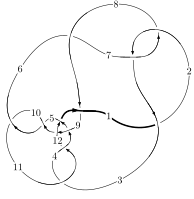
\includegraphics[width=112pt]{../../../GIT/diagram.site/Diagrams/png/1474_12a_0673.png}\\
\ \ \ A knot diagram\footnotemark}&
\allowdisplaybreaks
\textbf{Linearized knot diagam} \\
\cline{2-2}
 &
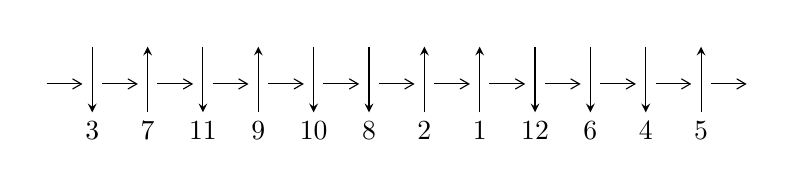
\begin{tikzpicture}[x=20pt, y=17pt]
	% nodes
	\node (C0) at (0, 0) {};
	\node (C1) at (1, 0) {};
	\node (C1U) at (1, +1) {};
	\node (C1D) at (1, -1) {3};

	\node (C2) at (2, 0) {};
	\node (C2U) at (2, +1) {};
	\node (C2D) at (2, -1) {7};

	\node (C3) at (3, 0) {};
	\node (C3U) at (3, +1) {};
	\node (C3D) at (3, -1) {11};

	\node (C4) at (4, 0) {};
	\node (C4U) at (4, +1) {};
	\node (C4D) at (4, -1) {9};

	\node (C5) at (5, 0) {};
	\node (C5U) at (5, +1) {};
	\node (C5D) at (5, -1) {10};

	\node (C6) at (6, 0) {};
	\node (C6U) at (6, +1) {};
	\node (C6D) at (6, -1) {8};

	\node (C7) at (7, 0) {};
	\node (C7U) at (7, +1) {};
	\node (C7D) at (7, -1) {2};

	\node (C8) at (8, 0) {};
	\node (C8U) at (8, +1) {};
	\node (C8D) at (8, -1) {1};

	\node (C9) at (9, 0) {};
	\node (C9U) at (9, +1) {};
	\node (C9D) at (9, -1) {12};

	\node (C10) at (10, 0) {};
	\node (C10U) at (10, +1) {};
	\node (C10D) at (10, -1) {6};

	\node (C11) at (11, 0) {};
	\node (C11U) at (11, +1) {};
	\node (C11D) at (11, -1) {4};

	\node (C12) at (12, 0) {};
	\node (C12U) at (12, +1) {};
	\node (C12D) at (12, -1) {5};
	\node (C13) at (13, 0) {};

	% arrows
	\draw[->,>={angle 60}]
	(C0) edge (C1) (C1) edge (C2) (C2) edge (C3) (C3) edge (C4) (C4) edge (C5) (C5) edge (C6) (C6) edge (C7) (C7) edge (C8) (C8) edge (C9) (C9) edge (C10) (C10) edge (C11) (C11) edge (C12) (C12) edge (C13) ;	\draw[->,>=stealth]
	(C1U) edge (C1D) (C2D) edge (C2U) (C3U) edge (C3D) (C4D) edge (C4U) (C5U) edge (C5D) (C6U) edge (C6D) (C7D) edge (C7U) (C8D) edge (C8U) (C9U) edge (C9D) (C10U) edge (C10D) (C11U) edge (C11D) (C12D) edge (C12U) ;
	\end{tikzpicture} \\
\hhline{~~} \\& 
\textbf{Solving Sequence} \\ \cline{2-2} 
 &
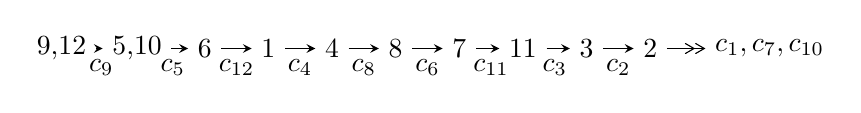
\begin{tikzpicture}[x=23pt, y=7pt]
	% node
	\node (A0) at (-1/8, 0) {9,12};
	\node (A1) at (17/16, 0) {5,10};
	\node (A2) at (17/8, 0) {6};
	\node (A3) at (25/8, 0) {1};
	\node (A4) at (33/8, 0) {4};
	\node (A5) at (41/8, 0) {8};
	\node (A6) at (49/8, 0) {7};
	\node (A7) at (57/8, 0) {11};
	\node (A8) at (65/8, 0) {3};
	\node (A9) at (73/8, 0) {2};
	\node (C1) at (1/2, -1) {$c_{9}$};
	\node (C2) at (13/8, -1) {$c_{5}$};
	\node (C3) at (21/8, -1) {$c_{12}$};
	\node (C4) at (29/8, -1) {$c_{4}$};
	\node (C5) at (37/8, -1) {$c_{8}$};
	\node (C6) at (45/8, -1) {$c_{6}$};
	\node (C7) at (53/8, -1) {$c_{11}$};
	\node (C8) at (61/8, -1) {$c_{3}$};
	\node (C9) at (69/8, -1) {$c_{2}$};
	\node (A10) at (11, 0) {$c_{1},c_{7},c_{10}$};

	% edge
	\draw[->,>=stealth]	
	(A0) edge (A1) (A1) edge (A2) (A2) edge (A3) (A3) edge (A4) (A4) edge (A5) (A5) edge (A6) (A6) edge (A7) (A7) edge (A8) (A8) edge (A9) ;
	\draw[->>,>={angle 60}]	
	(A9) edge (A10);
\end{tikzpicture} \\ 

\end{tabular} \\

\footnotetext{
The image of knot diagram is generated by the software ``\textbf{Draw programme}" developed by Andrew Bartholomew(\url{http://www.layer8.co.uk/maths/draw/index.htm\#Running-draw}), where we modified some parts for our purpose(\url{https://github.com/CATsTAILs/LinksPainter}).
}\phantom \\ \newline 
\centering \textbf{Ideals for irreducible components\footnotemark of $X_{\text{par}}$} 
 
\begin{align*}
I^u_{1}&=\langle 
-579387 u^{39}-23275447 u^{38}+\cdots+8192 b-8251727872,\\
\phantom{I^u_{1}}&\phantom{= \langle  }-1007291 u^{39}-40140157 u^{38}+\cdots+16384 a-16662396928,\\
\phantom{I^u_{1}}&\phantom{= \langle  }u^{40}+41 u^{39}+\cdots+401408 u+16384\rangle \\
I^u_{2}&=\langle 
-3.50204\times10^{97} a^{27} u^{2}+1.27267\times10^{97} a^{26} u^{2}+\cdots-3.32558\times10^{97} a-9.43161\times10^{94},\\
\phantom{I^u_{2}}&\phantom{= \langle  }a^{27} u^2-5 a^{26} u^2+\cdots+285596 a+148877,\;u^3- u^2+1\rangle \\
I^u_{3}&=\langle 
-13 u^{22}+66 u^{21}+\cdots+b+11,\;-11 u^{22}+53 u^{21}+\cdots+a+1,\;u^{23}-6 u^{22}+\cdots-4 u^2+1\rangle \\
\\
\end{align*}
\raggedright * 3 irreducible components of $\dim_{\mathbb{C}}=0$, with total 147 representations.\\
\footnotetext{All coefficients of polynomials are rational numbers. But the coefficients are sometimes approximated in decimal forms when there is not enough margin.}
\newpage
\renewcommand{\arraystretch}{1}
\centering \section*{I. $I^u_{1}= \langle -5.79\times10^{5} u^{39}-2.33\times10^{7} u^{38}+\cdots+8192 b-8.25\times10^{9},\;-1.01\times10^{6} u^{39}-4.01\times10^{7} u^{38}+\cdots+1.64\times10^{4} a-1.67\times10^{10},\;u^{40}+41 u^{39}+\cdots+401408 u+16384 \rangle$}
\flushleft \textbf{(i) Arc colorings}\\
\begin{tabular}{m{7pt} m{180pt} m{7pt} m{180pt} }
\flushright $a_{9}=$&$\begin{pmatrix}1\\0\end{pmatrix}$ \\
\flushright $a_{12}=$&$\begin{pmatrix}0\\u\end{pmatrix}$ \\
\flushright $a_{5}=$&$\begin{pmatrix}61.4802 u^{39}+2449.96 u^{38}+\cdots+2.36167\times10^{7} u+1016992\\70.7260 u^{39}+2841.24 u^{38}+\cdots+2.36616\times10^{7} u+1007291\end{pmatrix}$ \\
\flushright $a_{10}=$&$\begin{pmatrix}1\\u^2\end{pmatrix}$ \\
\flushright $a_{6}=$&$\begin{pmatrix}49.2772 u^{39}+2035.73 u^{38}+\cdots+2.73378\times10^{7} u+1168475\\-140.846 u^{39}-5495.21 u^{38}+\cdots-1.06948\times10^{7} u-403173\end{pmatrix}$ \\
\flushright $a_{1}=$&$\begin{pmatrix}-1.00781 u^{39}-40.3125 u^{38}+\cdots-386593 u-16447.5\\-1.00781 u^{39}-40.3203 u^{38}+\cdots-388096. u-16512\end{pmatrix}$ \\
\flushright $a_{4}=$&$\begin{pmatrix}-9.24579 u^{39}-391.280 u^{38}+\cdots-44895.3 u+9701\\70.7260 u^{39}+2841.24 u^{38}+\cdots+2.36616\times10^{7} u+1007291\end{pmatrix}$ \\
\flushright $a_{8}=$&$\begin{pmatrix}-8.96484 u^{39}-359.707 u^{38}+\cdots-3.84858\times10^{6} u-164479\\-6.85156 u^{39}-275.133 u^{38}+\cdots-3046048 u-130368\end{pmatrix}$ \\
\flushright $a_{7}=$&$\begin{pmatrix}115.111 u^{39}+4531.45 u^{38}+\cdots+1.61831\times10^{7} u+643411\\135.594 u^{39}+5527.05 u^{38}+\cdots+5.94395\times10^{7} u+2503924\end{pmatrix}$ \\
\flushright $a_{11}=$&$\begin{pmatrix}\frac{1}{128} u^{39}+\frac{5}{16} u^{38}+\cdots+1568 u+\frac{129}{2}\\-0.00781250 u^{39}-0.304688 u^{38}+\cdots-1503.50 u^{2}-63.5000 u\end{pmatrix}$ \\
\flushright $a_{3}=$&$\begin{pmatrix}-21.4449 u^{39}-742.195 u^{38}+\cdots+1.96811\times10^{7} u+856786.\\-128.012 u^{39}-5132.03 u^{38}+\cdots-3.03051\times10^{7} u-1238166\end{pmatrix}$ \\
\flushright $a_{2}=$&$\begin{pmatrix}-2.46484 u^{39}-99.5313 u^{38}+\cdots-783425. u-32640\\11.0078 u^{39}+439.559 u^{38}+\cdots+3859393 u+163968\end{pmatrix}$\\&\end{tabular}
\flushleft \textbf{(ii) Obstruction class $= -1$}\\~\\
\flushleft \textbf{(iii) Cusp Shapes $= \frac{313701}{2048} u^{39}+\frac{12529453}{2048} u^{38}+\cdots+15458438 u+553758$}\\~\\
\newpage\renewcommand{\arraystretch}{1}
\flushleft \textbf{(iv) u-Polynomials at the component}\newline \\
\begin{tabular}{m{50pt}|m{274pt}}
Crossings & \hspace{64pt}u-Polynomials at each crossing \\
\hline $$\begin{aligned}c_{1},c_{6}\end{aligned}$$&$\begin{aligned}
&u^{40}+13 u^{39}+\cdots+32 u+64
\end{aligned}$\\
\hline $$\begin{aligned}c_{2},c_{7}\end{aligned}$$&$\begin{aligned}
&u^{40}+7 u^{39}+\cdots+2 u^2+8
\end{aligned}$\\
\hline $$\begin{aligned}c_{3},c_{5},c_{10}\\c_{11}\end{aligned}$$&$\begin{aligned}
&u^{40}+u^{39}+\cdots+2 u+1
\end{aligned}$\\
\hline $$\begin{aligned}c_{4},c_{12}\end{aligned}$$&$\begin{aligned}
&u^{40}+3 u^{38}+\cdots+3 u+1
\end{aligned}$\\
\hline $$\begin{aligned}c_{8}\end{aligned}$$&$\begin{aligned}
&u^{40}-35 u^{39}+\cdots-4086976 u+307752
\end{aligned}$\\
\hline $$\begin{aligned}c_{9}\end{aligned}$$&$\begin{aligned}
&u^{40}-41 u^{39}+\cdots-401408 u+16384
\end{aligned}$\\
\hline
\end{tabular}\\~\\
\newpage\renewcommand{\arraystretch}{1}
\flushleft \textbf{(v) Riley Polynomials at the component}\newline \\
\begin{tabular}{m{50pt}|m{274pt}}
Crossings & \hspace{64pt}Riley Polynomials at each crossing \\
\hline $$\begin{aligned}c_{1},c_{6}\end{aligned}$$&$\begin{aligned}
&y^{40}+25 y^{39}+\cdots-27136 y+4096
\end{aligned}$\\
\hline $$\begin{aligned}c_{2},c_{7}\end{aligned}$$&$\begin{aligned}
&y^{40}+13 y^{39}+\cdots+32 y+64
\end{aligned}$\\
\hline $$\begin{aligned}c_{3},c_{5},c_{10}\\c_{11}\end{aligned}$$&$\begin{aligned}
&y^{40}-35 y^{39}+\cdots+20 y+1
\end{aligned}$\\
\hline $$\begin{aligned}c_{4},c_{12}\end{aligned}$$&$\begin{aligned}
&y^{40}+6 y^{39}+\cdots+5 y+1
\end{aligned}$\\
\hline $$\begin{aligned}c_{8}\end{aligned}$$&$\begin{aligned}
&y^{40}+17 y^{39}+\cdots+373353571616 y+94711293504
\end{aligned}$\\
\hline $$\begin{aligned}c_{9}\end{aligned}$$&$\begin{aligned}
&y^{40}-7 y^{39}+\cdots-1409286144 y+268435456
\end{aligned}$\\
\hline
\end{tabular}\\~\\
\newpage\flushleft \textbf{(vi) Complex Volumes and Cusp Shapes}
$$\begin{array}{c|c|c}  
\text{Solutions to }I^u_{1}& \I (\text{vol} + \sqrt{-1}CS) & \text{Cusp shape}\\
 \hline 
\begin{aligned}
u &= -0.386041 + 0.781738 I \\
a &= \phantom{-}0.327982 + 0.912189 I \\
b &= \phantom{-}0.839708 + 0.095747 I\end{aligned}
 & \phantom{-}4.29895 - 4.62297 I & \phantom{-0.000000 } 0 \\ \hline\begin{aligned}
u &= -0.386041 - 0.781738 I \\
a &= \phantom{-}0.327982 - 0.912189 I \\
b &= \phantom{-}0.839708 - 0.095747 I\end{aligned}
 & \phantom{-}4.29895 + 4.62297 I & \phantom{-0.000000 } 0 \\ \hline\begin{aligned}
u &= -0.424468 + 0.716698 I \\
a &= -0.337606 - 1.005260 I \\
b &= -0.863768 - 0.184738 I\end{aligned}
 & \phantom{-}4.71501 + 0.92897 I & \phantom{-0.000000 } 0 \\ \hline\begin{aligned}
u &= -0.424468 - 0.716698 I \\
a &= -0.337606 + 1.005260 I \\
b &= -0.863768 + 0.184738 I\end{aligned}
 & \phantom{-}4.71501 - 0.92897 I & \phantom{-0.000000 } 0 \\ \hline\begin{aligned}
u &= -0.688781 + 0.410406 I \\
a &= \phantom{-}0.50871 + 1.50198 I \\
b &= \phantom{-}0.966812 + 0.825756 I\end{aligned}
 & \phantom{-}2.54965 + 8.13634 I & \phantom{-0.000000 } 0 \\ \hline\begin{aligned}
u &= -0.688781 - 0.410406 I \\
a &= \phantom{-}0.50871 - 1.50198 I \\
b &= \phantom{-}0.966812 - 0.825756 I\end{aligned}
 & \phantom{-}2.54965 - 8.13634 I & \phantom{-0.000000 } 0 \\ \hline\begin{aligned}
u &= -0.654557 + 0.438339 I \\
a &= -0.47237 - 1.45216 I \\
b &= -0.945733 - 0.743460 I\end{aligned}
 & \phantom{-}3.41551 + 2.50598 I & \phantom{-0.000000 } 0 \\ \hline\begin{aligned}
u &= -0.654557 - 0.438339 I \\
a &= -0.47237 + 1.45216 I \\
b &= -0.945733 + 0.743460 I\end{aligned}
 & \phantom{-}3.41551 - 2.50598 I & \phantom{-0.000000 } 0 \\ \hline\begin{aligned}
u &= -0.607234 + 0.303704 I \\
a &= \phantom{-}0.34044 + 1.61539 I \\
b &= \phantom{-}0.697328 + 0.877527 I\end{aligned}
 & -2.53281 + 2.82471 I & \phantom{-0.000000 } 0 \\ \hline\begin{aligned}
u &= -0.607234 - 0.303704 I \\
a &= \phantom{-}0.34044 - 1.61539 I \\
b &= \phantom{-}0.697328 - 0.877527 I\end{aligned}
 & -2.53281 - 2.82471 I & \phantom{-0.000000 } 0\\
 \hline 
 \end{array}$$\newpage$$\begin{array}{c|c|c}  
\text{Solutions to }I^u_{1}& \I (\text{vol} + \sqrt{-1}CS) & \text{Cusp shape}\\
 \hline 
\begin{aligned}
u &= -0.445048 + 0.401866 I \\
a &= -0.184660 - 1.394420 I \\
b &= -0.642554 - 0.546377 I\end{aligned}
 & \phantom{-}1.01499 + 1.04142 I & \phantom{-0.000000 } 0 \\ \hline\begin{aligned}
u &= -0.445048 - 0.401866 I \\
a &= -0.184660 + 1.394420 I \\
b &= -0.642554 + 0.546377 I\end{aligned}
 & \phantom{-}1.01499 - 1.04142 I & \phantom{-0.000000 } 0 \\ \hline\begin{aligned}
u &= \phantom{-}0.079057 + 0.565866 I \\
a &= -0.254159 + 0.764745 I \\
b &= \phantom{-}0.452836 + 0.083361 I\end{aligned}
 & -0.513730 - 1.280700 I & \phantom{-0.000000 } 0 \\ \hline\begin{aligned}
u &= \phantom{-}0.079057 - 0.565866 I \\
a &= -0.254159 - 0.764745 I \\
b &= \phantom{-}0.452836 - 0.083361 I\end{aligned}
 & -0.513730 + 1.280700 I & \phantom{-0.000000 } 0 \\ \hline\begin{aligned}
u &= -0.530557 + 0.081357 I \\
a &= \phantom{-}0.07376 + 1.79161 I \\
b &= \phantom{-}0.184894 + 0.944550 I\end{aligned}
 & -0.04537 - 2.31418 I & \phantom{-0.000000 } 0 \\ \hline\begin{aligned}
u &= -0.530557 - 0.081357 I \\
a &= \phantom{-}0.07376 - 1.79161 I \\
b &= \phantom{-}0.184894 - 0.944550 I\end{aligned}
 & -0.04537 + 2.31418 I & \phantom{-0.000000 } 0 \\ \hline\begin{aligned}
u &= -1.29444 + 0.91899 I \\
a &= -0.059482 - 1.047590 I \\
b &= -1.03972 - 1.30139 I\end{aligned}
 & -7.1554 + 18.5968 I & \phantom{-0.000000 } 0 \\ \hline\begin{aligned}
u &= -1.29444 - 0.91899 I \\
a &= -0.059482 + 1.047590 I \\
b &= -1.03972 + 1.30139 I\end{aligned}
 & -7.1554 - 18.5968 I & \phantom{-0.000000 } 0 \\ \hline\begin{aligned}
u &= -1.30733 + 0.91344 I \\
a &= \phantom{-}0.076070 + 1.022580 I \\
b &= \phantom{-}1.03351 + 1.26737 I\end{aligned}
 & -5.82110 + 12.79620 I & \phantom{-0.000000 } 0 \\ \hline\begin{aligned}
u &= -1.30733 - 0.91344 I \\
a &= \phantom{-}0.076070 - 1.022580 I \\
b &= \phantom{-}1.03351 - 1.26737 I\end{aligned}
 & -5.82110 - 12.79620 I & \phantom{-0.000000 } 0\\
 \hline 
 \end{array}$$\newpage$$\begin{array}{c|c|c}  
\text{Solutions to }I^u_{1}& \I (\text{vol} + \sqrt{-1}CS) & \text{Cusp shape}\\
 \hline 
\begin{aligned}
u &= -1.31965 + 0.94989 I \\
a &= -0.009169 - 0.979688 I \\
b &= -0.94269 - 1.28413 I\end{aligned}
 & -12.4391 + 11.8677 I & \phantom{-0.000000 } 0 \\ \hline\begin{aligned}
u &= -1.31965 - 0.94989 I \\
a &= -0.009169 + 0.979688 I \\
b &= -0.94269 + 1.28413 I\end{aligned}
 & -12.4391 - 11.8677 I & \phantom{-0.000000 } 0 \\ \hline\begin{aligned}
u &= -1.36530 + 0.94019 I \\
a &= \phantom{-}0.052407 + 0.903121 I \\
b &= \phantom{-}0.92065 + 1.18375 I\end{aligned}
 & -7.44660 + 9.43936 I & \phantom{-0.000000 } 0 \\ \hline\begin{aligned}
u &= -1.36530 - 0.94019 I \\
a &= \phantom{-}0.052407 - 0.903121 I \\
b &= \phantom{-}0.92065 - 1.18375 I\end{aligned}
 & -7.44660 - 9.43936 I & \phantom{-0.000000 } 0 \\ \hline\begin{aligned}
u &= -1.37313 + 0.98630 I \\
a &= \phantom{-}0.016734 - 0.861988 I \\
b &= -0.82720 - 1.20013 I\end{aligned}
 & -9.66748 + 4.61526 I & \phantom{-0.000000 } 0 \\ \hline\begin{aligned}
u &= -1.37313 - 0.98630 I \\
a &= \phantom{-}0.016734 + 0.861988 I \\
b &= -0.82720 + 1.20013 I\end{aligned}
 & -9.66748 - 4.61526 I & \phantom{-0.000000 } 0 \\ \hline\begin{aligned}
u &= -1.58176 + 0.75718 I \\
a &= \phantom{-}0.318816 + 0.640437 I \\
b &= \phantom{-}0.989214 + 0.771613 I\end{aligned}
 & \phantom{-}0.26052 + 9.55635 I & \phantom{-0.000000 } 0 \\ \hline\begin{aligned}
u &= -1.58176 - 0.75718 I \\
a &= \phantom{-}0.318816 - 0.640437 I \\
b &= \phantom{-}0.989214 - 0.771613 I\end{aligned}
 & \phantom{-}0.26052 - 9.55635 I & \phantom{-0.000000 } 0 \\ \hline\begin{aligned}
u &= -1.67866 + 0.73710 I \\
a &= -0.323543 - 0.544420 I \\
b &= -0.944411 - 0.675412 I\end{aligned}
 & \phantom{-}0.62354 + 3.38801 I & \phantom{-0.000000 } 0 \\ \hline\begin{aligned}
u &= -1.67866 - 0.73710 I \\
a &= -0.323543 + 0.544420 I \\
b &= -0.944411 + 0.675412 I\end{aligned}
 & \phantom{-}0.62354 - 3.38801 I & \phantom{-0.000000 } 0\\
 \hline 
 \end{array}$$\newpage$$\begin{array}{c|c|c}  
\text{Solutions to }I^u_{1}& \I (\text{vol} + \sqrt{-1}CS) & \text{Cusp shape}\\
 \hline 
\begin{aligned}
u &= -0.91638 + 1.89680 I \\
a &= -0.306375 + 0.043826 I \\
b &= -0.197627 + 0.621294 I\end{aligned}
 & -4.94081 - 9.75847 I & \phantom{-0.000000 } 0 \\ \hline\begin{aligned}
u &= -0.91638 - 1.89680 I \\
a &= -0.306375 - 0.043826 I \\
b &= -0.197627 - 0.621294 I\end{aligned}
 & -4.94081 + 9.75847 I & \phantom{-0.000000 } 0 \\ \hline\begin{aligned}
u &= -1.66153 + 1.30418 I \\
a &= -0.074448 + 0.424186 I \\
b &= \phantom{-}0.429519 + 0.801889 I\end{aligned}
 & -8.50425 + 5.60885 I & \phantom{-0.000000 } 0 \\ \hline\begin{aligned}
u &= -1.66153 - 1.30418 I \\
a &= -0.074448 - 0.424186 I \\
b &= \phantom{-}0.429519 - 0.801889 I\end{aligned}
 & -8.50425 - 5.60885 I & \phantom{-0.000000 } 0 \\ \hline\begin{aligned}
u &= -1.43142 + 1.78513 I \\
a &= -0.217267 + 0.216904 I \\
b &= \phantom{-}0.076202 + 0.698329 I\end{aligned}
 & -10.59290 - 2.39404 I & \phantom{-0.000000 } 0 \\ \hline\begin{aligned}
u &= -1.43142 - 1.78513 I \\
a &= -0.217267 - 0.216904 I \\
b &= \phantom{-}0.076202 - 0.698329 I\end{aligned}
 & -10.59290 + 2.39404 I & \phantom{-0.000000 } 0 \\ \hline\begin{aligned}
u &= -0.94045 + 2.13875 I \\
a &= \phantom{-}0.233463 - 0.037102 I \\
b &= \phantom{-}0.140206 - 0.534212 I\end{aligned}
 & -3.38165 - 3.78335 I & \phantom{-0.000000 } 0 \\ \hline\begin{aligned}
u &= -0.94045 - 2.13875 I \\
a &= \phantom{-}0.233463 + 0.037102 I \\
b &= \phantom{-}0.140206 + 0.534212 I\end{aligned}
 & -3.38165 + 3.78335 I & \phantom{-0.000000 } 0 \\ \hline\begin{aligned}
u &= -1.97234 + 1.58931 I \\
a &= \phantom{-}0.040698 - 0.256368 I \\
b &= -0.327178 - 0.570325 I\end{aligned}
 & -5.52208 + 0.87397 I & \phantom{-0.000000 } 0 \\ \hline\begin{aligned}
u &= -1.97234 - 1.58931 I \\
a &= \phantom{-}0.040698 + 0.256368 I \\
b &= -0.327178 + 0.570325 I\end{aligned}
 & -5.52208 - 0.87397 I & \phantom{-0.000000 } 0\\
 \hline 
 \end{array}$$\newpage\newpage\renewcommand{\arraystretch}{1}
\centering \section*{II. $I^u_{2}= \langle -3.50\times10^{97} a^{27} u^{2}+1.27\times10^{97} a^{26} u^{2}+\cdots-3.33\times10^{97} a-9.43\times10^{94},\;a^{27} u^2-5 a^{26} u^2+\cdots+285596 a+148877,\;u^3- u^2+1 \rangle$}
\flushleft \textbf{(i) Arc colorings}\\
\begin{tabular}{m{7pt} m{180pt} m{7pt} m{180pt} }
\flushright $a_{9}=$&$\begin{pmatrix}1\\0\end{pmatrix}$ \\
\flushright $a_{12}=$&$\begin{pmatrix}0\\u\end{pmatrix}$ \\
\flushright $a_{5}=$&$\begin{pmatrix}a\\10.2657 a^{27} u^{2}-3.73064 a^{26} u^{2}+\cdots+9.74846 a+0.0276474\end{pmatrix}$ \\
\flushright $a_{10}=$&$\begin{pmatrix}1\\u^2\end{pmatrix}$ \\
\flushright $a_{6}=$&$\begin{pmatrix}-10.2657 a^{27} u^{2}+3.73064 a^{26} u^{2}+\cdots-8.74846 a-0.0276474\\17.0710 a^{27} u^{2}-5.63123 a^{26} u^{2}+\cdots-1.53110 a-0.821207\end{pmatrix}$ \\
\flushright $a_{1}=$&$\begin{pmatrix}a^2 u\\-2.14419 a^{27} u^{2}-3.82791 a^{26} u^{2}+\cdots+14.6111 a+5.85525\end{pmatrix}$ \\
\flushright $a_{4}=$&$\begin{pmatrix}-10.2657 a^{27} u^{2}+3.73064 a^{26} u^{2}+\cdots-8.74846 a-0.0276474\\10.2657 a^{27} u^{2}-3.73064 a^{26} u^{2}+\cdots+9.74846 a+0.0276474\end{pmatrix}$ \\
\flushright $a_{8}=$&$\begin{pmatrix}3.13258 a^{27} u^{2}+1.11366 a^{26} u^{2}+\cdots+8.60740 a+4.83529\\-2.20805 a^{27} u^{2}+3.25415 a^{26} u^{2}+\cdots+6.88820 a-1.57925\end{pmatrix}$ \\
\flushright $a_{7}=$&$\begin{pmatrix}-17.2876 a^{27} u^{2}+3.16256 a^{26} u^{2}+\cdots-22.6088 a-10.3492\\3.39639 a^{27} u^{2}-2.26539 a^{26} u^{2}+\cdots-5.45361 a+4.59514\end{pmatrix}$ \\
\flushright $a_{11}=$&$\begin{pmatrix}-5.04547 a^{27} u^{2}+8.36584 a^{26} u^{2}+\cdots+5.97337 a+0.330067\\7.18966 a^{27} u^{2}-4.53793 a^{26} u^{2}+\cdots-20.5845 a-6.18532\end{pmatrix}$ \\
\flushright $a_{3}=$&$\begin{pmatrix}-5.05099 a^{27} u^{2}-0.537079 a^{26} u^{2}+\cdots+17.4477 a+3.50841\\-13.3963 a^{27} u^{2}+8.75813 a^{26} u^{2}+\cdots-5.43958 a-4.39989\end{pmatrix}$ \\
\flushright $a_{2}=$&$\begin{pmatrix}2.77771 a^{27} u^{2}-7.24386 a^{26} u^{2}+\cdots+19.9178 a+0.0502453\\-16.1715 a^{27} u^{2}+19.3292 a^{26} u^{2}+\cdots-8.66336 a-1.90620\end{pmatrix}$\\&\end{tabular}
\flushleft \textbf{(ii) Obstruction class $= -1$}\\~\\
\flushleft \textbf{(iii) Cusp Shapes $= 135.121 a^{27} u^{2}-4.70834 a^{26} u^{2}+\cdots-47.4051 a-38.0609$}\\~\\
\newpage\renewcommand{\arraystretch}{1}
\flushleft \textbf{(iv) u-Polynomials at the component}\newline \\
\begin{tabular}{m{50pt}|m{274pt}}
Crossings & \hspace{64pt}u-Polynomials at each crossing \\
\hline $$\begin{aligned}c_{1},c_{6},c_{8}\end{aligned}$$&$\begin{aligned}
&(u^{14}+5 u^{13}+\cdots+3 u+1)^{6}
\end{aligned}$\\
\hline $$\begin{aligned}c_{2},c_{7}\end{aligned}$$&$\begin{aligned}
&(u^{14}- u^{13}+\cdots+u+1)^{6}
\end{aligned}$\\
\hline $$\begin{aligned}c_{3},c_{5},c_{10}\\c_{11}\end{aligned}$$&$\begin{aligned}
&u^{84}- u^{83}+\cdots-36600 u+3721
\end{aligned}$\\
\hline $$\begin{aligned}c_{4},c_{12}\end{aligned}$$&$\begin{aligned}
&u^{84}-3 u^{83}+\cdots-16116 u+6737
\end{aligned}$\\
\hline $$\begin{aligned}c_{9}\end{aligned}$$&$\begin{aligned}
&(u^3+u^2-1)^{28}
\end{aligned}$\\
\hline
\end{tabular}\\~\\
\newpage\renewcommand{\arraystretch}{1}
\flushleft \textbf{(v) Riley Polynomials at the component}\newline \\
\begin{tabular}{m{50pt}|m{274pt}}
Crossings & \hspace{64pt}Riley Polynomials at each crossing \\
\hline $$\begin{aligned}c_{1},c_{6},c_{8}\end{aligned}$$&$\begin{aligned}
&(y^{14}+9 y^{13}+\cdots+15 y+1)^{6}
\end{aligned}$\\
\hline $$\begin{aligned}c_{2},c_{7}\end{aligned}$$&$\begin{aligned}
&(y^{14}+5 y^{13}+\cdots+3 y+1)^{6}
\end{aligned}$\\
\hline $$\begin{aligned}c_{3},c_{5},c_{10}\\c_{11}\end{aligned}$$&$\begin{aligned}
&y^{84}-69 y^{83}+\cdots+118923160 y+13845841
\end{aligned}$\\
\hline $$\begin{aligned}c_{4},c_{12}\end{aligned}$$&$\begin{aligned}
&y^{84}+23 y^{83}+\cdots+2095745328 y+45387169
\end{aligned}$\\
\hline $$\begin{aligned}c_{9}\end{aligned}$$&$\begin{aligned}
&(y^3- y^2+2 y-1)^{28}
\end{aligned}$\\
\hline
\end{tabular}\\~\\
\newpage\flushleft \textbf{(vi) Complex Volumes and Cusp Shapes}
$$\begin{array}{c|c|c}  
\text{Solutions to }I^u_{2}& \I (\text{vol} + \sqrt{-1}CS) & \text{Cusp shape}\\
 \hline 
\begin{aligned}
u &= \phantom{-}0.877439 + 0.744862 I \\
a &= -0.120006 - 0.991776 I \\
b &= \phantom{-}0.72497 - 1.60540 I\end{aligned}
 & -3.10096 + 0.58459 I & -6.59625 + 0.35429 I \\ \hline\begin{aligned}
u &= \phantom{-}0.877439 + 0.744862 I \\
a &= \phantom{-}0.986237 - 0.087553 I \\
b &= \phantom{-}0.123059 + 0.619630 I\end{aligned}
 & -1.91067 + 6.10773 I & -4.49024 - 4.28133 I \\ \hline\begin{aligned}
u &= \phantom{-}0.877439 + 0.744862 I \\
a &= -0.006942 - 0.989783 I \\
b &= \phantom{-}0.96956 - 1.57337 I\end{aligned}
 & -6.55340 - 5.59559 I & -9.90787 + 6.19322 I \\ \hline\begin{aligned}
u &= \phantom{-}0.877439 + 0.744862 I \\
a &= \phantom{-}0.084543 - 0.980700 I \\
b &= \phantom{-}1.15049 - 1.52825 I\end{aligned}
 & -1.91067 - 11.76400 I & -4.49024 + 10.24022 I \\ \hline\begin{aligned}
u &= \phantom{-}0.877439 + 0.744862 I \\
a &= \phantom{-}0.954989 + 0.177300 I \\
b &= -0.023799 + 0.748491 I\end{aligned}
 & -6.55340 - 0.06065 I & -9.90787 - 0.23433 I \\ \hline\begin{aligned}
u &= \phantom{-}0.877439 + 0.744862 I \\
a &= \phantom{-}0.929113 + 0.489507 I \\
b &= -0.162423 + 0.898869 I\end{aligned}
 & -3.10096 - 6.24083 I & -6.59625 + 5.60461 I \\ \hline\begin{aligned}
u &= \phantom{-}0.877439 + 0.744862 I \\
a &= -0.075925 + 0.944213 I \\
b &= -1.12272 + 1.45979 I\end{aligned}
 & -0.72038 - 6.24083 I & -2.38424 + 5.60461 I \\ \hline\begin{aligned}
u &= \phantom{-}0.877439 + 0.744862 I \\
a &= -0.345086 + 1.036840 I \\
b &= -0.452684 + 0.317394 I\end{aligned}
 & \phantom{-}2.73205 - 0.06065 I & \phantom{-}0.927378 - 0.234326 I \\ \hline\begin{aligned}
u &= \phantom{-}0.877439 + 0.744862 I \\
a &= \phantom{-}0.178079 + 0.886248 I \\
b &= -0.58485 + 1.35446 I\end{aligned}
 & -1.93349 - 4.20582 I & -5.37614 + 7.10152 I \\ \hline\begin{aligned}
u &= \phantom{-}0.877439 + 0.744862 I \\
a &= -0.633327 - 0.629672 I \\
b &= \phantom{-}0.343438 - 0.886961 I\end{aligned}
 & -1.93349 - 1.45042 I & -5.37614 - 1.14262 I\\
 \hline 
 \end{array}$$\newpage$$\begin{array}{c|c|c}  
\text{Solutions to }I^u_{2}& \I (\text{vol} + \sqrt{-1}CS) & \text{Cusp shape}\\
 \hline 
\begin{aligned}
u &= \phantom{-}0.877439 + 0.744862 I \\
a &= -0.873175 + 0.094296 I \\
b &= -0.063434 - 0.555802 I\end{aligned}
 & -0.720385 + 0.584589 I & -2.38424 + 0.35429 I \\ \hline\begin{aligned}
u &= \phantom{-}0.877439 + 0.744862 I \\
a &= \phantom{-}0.095249 + 0.871209 I \\
b &= -0.77182 + 1.33732 I\end{aligned}
 & -1.88785 - 4.20582 I & -3.60435 + 7.10152 I \\ \hline\begin{aligned}
u &= \phantom{-}0.877439 + 0.744862 I \\
a &= \phantom{-}0.271240 + 0.780595 I \\
b &= \phantom{-}0.086688 + 1.024240 I\end{aligned}
 & -1.93349 - 1.45042 I & -5.37614 - 1.14262 I \\ \hline\begin{aligned}
u &= \phantom{-}0.877439 + 0.744862 I \\
a &= \phantom{-}0.297573 - 1.147490 I \\
b &= \phantom{-}0.527326 - 0.393396 I\end{aligned}
 & \phantom{-}2.73205 - 5.59559 I & \phantom{-}0.92738 + 6.19322 I \\ \hline\begin{aligned}
u &= \phantom{-}0.877439 + 0.744862 I \\
a &= -0.397833 - 0.686701 I \\
b &= -0.450625 - 1.121570 I\end{aligned}
 & -3.10096 - 6.24083 I & -6.59625 + 5.60461 I \\ \hline\begin{aligned}
u &= \phantom{-}0.877439 + 0.744862 I \\
a &= -0.601889 - 0.410389 I \\
b &= \phantom{-}0.317647 - 0.754765 I\end{aligned}
 & -1.88785 - 1.45042 I & -3.60435 - 1.14262 I \\ \hline\begin{aligned}
u &= \phantom{-}0.877439 + 0.744862 I \\
a &= -0.374205 - 1.225980 I \\
b &= \phantom{-}0.503878 - 0.910272 I\end{aligned}
 & -1.93349 - 4.20582 I & -5.37614 + 7.10152 I \\ \hline\begin{aligned}
u &= \phantom{-}0.877439 + 0.744862 I \\
a &= \phantom{-}0.213993 + 0.678532 I \\
b &= \phantom{-}0.222438 + 0.808416 I\end{aligned}
 & -1.88785 - 1.45042 I & -3.60435 - 1.14262 I \\ \hline\begin{aligned}
u &= \phantom{-}0.877439 + 0.744862 I \\
a &= -0.240729 - 1.319760 I \\
b &= \phantom{-}0.565355 - 0.835380 I\end{aligned}
 & -1.88785 - 4.20582 I & -3.60435 + 7.10152 I \\ \hline\begin{aligned}
u &= \phantom{-}0.877439 + 0.744862 I \\
a &= -0.405098 - 0.509151 I \\
b &= -0.705881 - 0.866905 I\end{aligned}
 & -6.55340 - 0.06065 I & -9.90787 - 0.23433 I\\
 \hline 
 \end{array}$$\newpage$$\begin{array}{c|c|c}  
\text{Solutions to }I^u_{2}& \I (\text{vol} + \sqrt{-1}CS) & \text{Cusp shape}\\
 \hline 
\begin{aligned}
u &= \phantom{-}0.877439 + 0.744862 I \\
a &= -0.128081 + 0.557074 I \\
b &= -1.115820 + 0.785201 I\end{aligned}
 & \phantom{-}2.73205 - 5.59559 I & \phantom{-}0.92738 + 6.19322 I \\ \hline\begin{aligned}
u &= \phantom{-}0.877439 + 0.744862 I \\
a &= -0.429915 - 0.341224 I \\
b &= -0.930577 - 0.657788 I\end{aligned}
 & -1.91067 + 6.10773 I & -4.49024 - 4.28133 I \\ \hline\begin{aligned}
u &= \phantom{-}0.877439 + 0.744862 I \\
a &= \phantom{-}0.354532 + 0.332473 I \\
b &= \phantom{-}0.836395 + 0.567656 I\end{aligned}
 & -0.720385 + 0.584589 I & -2.38424 + 0.35429 I \\ \hline\begin{aligned}
u &= \phantom{-}0.877439 + 0.744862 I \\
a &= \phantom{-}0.121375 - 0.464764 I \\
b &= \phantom{-}1.075100 - 0.652723 I\end{aligned}
 & \phantom{-}2.73205 - 0.06065 I & \phantom{-}0.927378 - 0.234326 I \\ \hline\begin{aligned}
u &= \phantom{-}0.877439 + 0.744862 I \\
a &= \phantom{-}0.42250 + 1.47099 I \\
b &= -0.633438 + 0.959610 I\end{aligned}
 & -3.10096 + 0.58459 I & \phantom{-0.000000 } 0 \\ \hline\begin{aligned}
u &= \phantom{-}0.877439 + 0.744862 I \\
a &= -0.07716 - 1.59819 I \\
b &= \phantom{-}0.769927 - 0.771935 I\end{aligned}
 & -0.72038 - 6.24083 I & \phantom{-0.000000 } 0 \\ \hline\begin{aligned}
u &= \phantom{-}0.877439 + 0.744862 I \\
a &= \phantom{-}0.24248 + 1.58730 I \\
b &= -0.731161 + 0.873645 I\end{aligned}
 & -6.55340 - 5.59559 I & \phantom{-0.000000 } 0 \\ \hline\begin{aligned}
u &= \phantom{-}0.877439 + 0.744862 I \\
a &= \phantom{-}0.09727 + 1.65915 I \\
b &= -0.804668 + 0.797531 I\end{aligned}
 & -1.91067 - 11.76400 I & \phantom{-0.000000 } 0 \\ \hline\begin{aligned}
u &= \phantom{-}0.877439 - 0.744862 I \\
a &= -0.120006 + 0.991776 I \\
b &= \phantom{-}0.72497 + 1.60540 I\end{aligned}
 & -3.10096 - 0.58459 I & -6.59625 - 0.35429 I \\ \hline\begin{aligned}
u &= \phantom{-}0.877439 - 0.744862 I \\
a &= \phantom{-}0.986237 + 0.087553 I \\
b &= \phantom{-}0.123059 - 0.619630 I\end{aligned}
 & -1.91067 - 6.10773 I & -4.49024 + 4.28133 I\\
 \hline 
 \end{array}$$\newpage$$\begin{array}{c|c|c}  
\text{Solutions to }I^u_{2}& \I (\text{vol} + \sqrt{-1}CS) & \text{Cusp shape}\\
 \hline 
\begin{aligned}
u &= \phantom{-}0.877439 - 0.744862 I \\
a &= -0.006942 + 0.989783 I \\
b &= \phantom{-}0.96956 + 1.57337 I\end{aligned}
 & -6.55340 + 5.59559 I & -9.90787 - 6.19322 I \\ \hline\begin{aligned}
u &= \phantom{-}0.877439 - 0.744862 I \\
a &= \phantom{-}0.084543 + 0.980700 I \\
b &= \phantom{-}1.15049 + 1.52825 I\end{aligned}
 & -1.91067 + 11.76400 I & -4.49024 - 10.24022 I \\ \hline\begin{aligned}
u &= \phantom{-}0.877439 - 0.744862 I \\
a &= \phantom{-}0.954989 - 0.177300 I \\
b &= -0.023799 - 0.748491 I\end{aligned}
 & -6.55340 + 0.06065 I & -9.90787 + 0.23433 I \\ \hline\begin{aligned}
u &= \phantom{-}0.877439 - 0.744862 I \\
a &= \phantom{-}0.929113 - 0.489507 I \\
b &= -0.162423 - 0.898869 I\end{aligned}
 & -3.10096 + 6.24083 I & -6.59625 - 5.60461 I \\ \hline\begin{aligned}
u &= \phantom{-}0.877439 - 0.744862 I \\
a &= -0.075925 - 0.944213 I \\
b &= -1.12272 - 1.45979 I\end{aligned}
 & -0.72038 + 6.24083 I & -2.38424 - 5.60461 I \\ \hline\begin{aligned}
u &= \phantom{-}0.877439 - 0.744862 I \\
a &= -0.345086 - 1.036840 I \\
b &= -0.452684 - 0.317394 I\end{aligned}
 & \phantom{-}2.73205 + 0.06065 I & \phantom{-}0.927378 + 0.234326 I \\ \hline\begin{aligned}
u &= \phantom{-}0.877439 - 0.744862 I \\
a &= \phantom{-}0.178079 - 0.886248 I \\
b &= -0.58485 - 1.35446 I\end{aligned}
 & -1.93349 + 4.20582 I & -5.37614 - 7.10152 I \\ \hline\begin{aligned}
u &= \phantom{-}0.877439 - 0.744862 I \\
a &= -0.633327 + 0.629672 I \\
b &= \phantom{-}0.343438 + 0.886961 I\end{aligned}
 & -1.93349 + 1.45042 I & -5.37614 + 1.14262 I \\ \hline\begin{aligned}
u &= \phantom{-}0.877439 - 0.744862 I \\
a &= -0.873175 - 0.094296 I \\
b &= -0.063434 + 0.555802 I\end{aligned}
 & -0.720385 - 0.584589 I & -2.38424 - 0.35429 I \\ \hline\begin{aligned}
u &= \phantom{-}0.877439 - 0.744862 I \\
a &= \phantom{-}0.095249 - 0.871209 I \\
b &= -0.77182 - 1.33732 I\end{aligned}
 & -1.88785 + 4.20582 I & -3.60435 - 7.10152 I\\
 \hline 
 \end{array}$$\newpage$$\begin{array}{c|c|c}  
\text{Solutions to }I^u_{2}& \I (\text{vol} + \sqrt{-1}CS) & \text{Cusp shape}\\
 \hline 
\begin{aligned}
u &= \phantom{-}0.877439 - 0.744862 I \\
a &= \phantom{-}0.271240 - 0.780595 I \\
b &= \phantom{-}0.086688 - 1.024240 I\end{aligned}
 & -1.93349 + 1.45042 I & -5.37614 + 1.14262 I \\ \hline\begin{aligned}
u &= \phantom{-}0.877439 - 0.744862 I \\
a &= \phantom{-}0.297573 + 1.147490 I \\
b &= \phantom{-}0.527326 + 0.393396 I\end{aligned}
 & \phantom{-}2.73205 + 5.59559 I & \phantom{-}0.92738 - 6.19322 I \\ \hline\begin{aligned}
u &= \phantom{-}0.877439 - 0.744862 I \\
a &= -0.397833 + 0.686701 I \\
b &= -0.450625 + 1.121570 I\end{aligned}
 & -3.10096 + 6.24083 I & -6.59625 - 5.60461 I \\ \hline\begin{aligned}
u &= \phantom{-}0.877439 - 0.744862 I \\
a &= -0.601889 + 0.410389 I \\
b &= \phantom{-}0.317647 + 0.754765 I\end{aligned}
 & -1.88785 + 1.45042 I & -3.60435 + 1.14262 I \\ \hline\begin{aligned}
u &= \phantom{-}0.877439 - 0.744862 I \\
a &= -0.374205 + 1.225980 I \\
b &= \phantom{-}0.503878 + 0.910272 I\end{aligned}
 & -1.93349 + 4.20582 I & -5.37614 - 7.10152 I \\ \hline\begin{aligned}
u &= \phantom{-}0.877439 - 0.744862 I \\
a &= \phantom{-}0.213993 - 0.678532 I \\
b &= \phantom{-}0.222438 - 0.808416 I\end{aligned}
 & -1.88785 + 1.45042 I & -3.60435 + 1.14262 I \\ \hline\begin{aligned}
u &= \phantom{-}0.877439 - 0.744862 I \\
a &= -0.240729 + 1.319760 I \\
b &= \phantom{-}0.565355 + 0.835380 I\end{aligned}
 & -1.88785 + 4.20582 I & -3.60435 - 7.10152 I \\ \hline\begin{aligned}
u &= \phantom{-}0.877439 - 0.744862 I \\
a &= -0.405098 + 0.509151 I \\
b &= -0.705881 + 0.866905 I\end{aligned}
 & -6.55340 + 0.06065 I & -9.90787 + 0.23433 I \\ \hline\begin{aligned}
u &= \phantom{-}0.877439 - 0.744862 I \\
a &= -0.128081 - 0.557074 I \\
b &= -1.115820 - 0.785201 I\end{aligned}
 & \phantom{-}2.73205 + 5.59559 I & \phantom{-}0.92738 - 6.19322 I \\ \hline\begin{aligned}
u &= \phantom{-}0.877439 - 0.744862 I \\
a &= -0.429915 + 0.341224 I \\
b &= -0.930577 + 0.657788 I\end{aligned}
 & -1.91067 - 6.10773 I & -4.49024 + 4.28133 I\\
 \hline 
 \end{array}$$\newpage$$\begin{array}{c|c|c}  
\text{Solutions to }I^u_{2}& \I (\text{vol} + \sqrt{-1}CS) & \text{Cusp shape}\\
 \hline 
\begin{aligned}
u &= \phantom{-}0.877439 - 0.744862 I \\
a &= \phantom{-}0.354532 - 0.332473 I \\
b &= \phantom{-}0.836395 - 0.567656 I\end{aligned}
 & -0.720385 - 0.584589 I & -2.38424 - 0.35429 I \\ \hline\begin{aligned}
u &= \phantom{-}0.877439 - 0.744862 I \\
a &= \phantom{-}0.121375 + 0.464764 I \\
b &= \phantom{-}1.075100 + 0.652723 I\end{aligned}
 & \phantom{-}2.73205 + 0.06065 I & \phantom{-}0.927378 + 0.234326 I \\ \hline\begin{aligned}
u &= \phantom{-}0.877439 - 0.744862 I \\
a &= \phantom{-}0.42250 - 1.47099 I \\
b &= -0.633438 - 0.959610 I\end{aligned}
 & -3.10096 - 0.58459 I & \phantom{-0.000000 } 0 \\ \hline\begin{aligned}
u &= \phantom{-}0.877439 - 0.744862 I \\
a &= -0.07716 + 1.59819 I \\
b &= \phantom{-}0.769927 + 0.771935 I\end{aligned}
 & -0.72038 + 6.24083 I & \phantom{-0.000000 } 0 \\ \hline\begin{aligned}
u &= \phantom{-}0.877439 - 0.744862 I \\
a &= \phantom{-}0.24248 - 1.58730 I \\
b &= -0.731161 - 0.873645 I\end{aligned}
 & -6.55340 + 5.59559 I & \phantom{-0.000000 } 0 \\ \hline\begin{aligned}
u &= \phantom{-}0.877439 - 0.744862 I \\
a &= \phantom{-}0.09727 - 1.65915 I \\
b &= -0.804668 - 0.797531 I\end{aligned}
 & -1.91067 + 11.76400 I & \phantom{-0.000000 } 0 \\ \hline\begin{aligned}
u &= -0.754878\phantom{ +0.000000I} \\
a &= \phantom{-}0.023468 + 0.988160 I \\
b &= -1.70900 + 1.25529 I\end{aligned}
 & -10.69100 + 2.76747 I & -16.4371 - 3.2138 I \\ \hline\begin{aligned}
u &= -0.754878\phantom{ +0.000000I} \\
a &= \phantom{-}0.023468 - 0.988160 I \\
b &= -1.70900 - 1.25529 I\end{aligned}
 & -10.69100 - 2.76747 I & -16.4371 + 3.2138 I \\ \hline\begin{aligned}
u &= -0.754878\phantom{ +0.000000I} \\
a &= -0.351285 + 0.840493 I \\
b &= \phantom{-}1.41371 + 0.90881 I\end{aligned}
 & -6.02544 - 1.37770 I & -10.13361 + 4.12207 I \\ \hline\begin{aligned}
u &= -0.754878\phantom{ +0.000000I} \\
a &= -0.351285 - 0.840493 I \\
b &= \phantom{-}1.41371 - 0.90881 I\end{aligned}
 & -6.02544 + 1.37770 I & -10.13361 - 4.12207 I\\
 \hline 
 \end{array}$$\newpage$$\begin{array}{c|c|c}  
\text{Solutions to }I^u_{2}& \I (\text{vol} + \sqrt{-1}CS) & \text{Cusp shape}\\
 \hline 
\begin{aligned}
u &= -0.754878\phantom{ +0.000000I} \\
a &= \phantom{-}0.010172 + 1.172770 I \\
b &= -1.59712 + 1.49891 I\end{aligned}
 & -6.04826 + 8.93586 I & -11.01951 - 7.26077 I \\ \hline\begin{aligned}
u &= -0.754878\phantom{ +0.000000I} \\
a &= \phantom{-}0.010172 - 1.172770 I \\
b &= -1.59712 - 1.49891 I\end{aligned}
 & -6.04826 - 8.93586 I & -11.01951 + 7.26077 I \\ \hline\begin{aligned}
u &= -0.754878\phantom{ +0.000000I} \\
a &= -0.082088 + 1.172510 I \\
b &= \phantom{-}1.50842 + 1.44210 I\end{aligned}
 & -4.85797 - 3.41271 I & -8.91351 + 2.62516 I \\ \hline\begin{aligned}
u &= -0.754878\phantom{ +0.000000I} \\
a &= -0.082088 - 1.172510 I \\
b &= \phantom{-}1.50842 - 1.44210 I\end{aligned}
 & -4.85797 + 3.41271 I & -8.91351 - 2.62516 I \\ \hline\begin{aligned}
u &= -0.754878\phantom{ +0.000000I} \\
a &= \phantom{-}0.039321 + 0.722074 I \\
b &= -1.82506 + 0.91144 I\end{aligned}
 & -7.23855 - 3.41271 I & -13.12551 + 2.62516 I \\ \hline\begin{aligned}
u &= -0.754878\phantom{ +0.000000I} \\
a &= \phantom{-}0.039321 - 0.722074 I \\
b &= -1.82506 - 0.91144 I\end{aligned}
 & -7.23855 + 3.41271 I & -13.12551 - 2.62516 I \\ \hline\begin{aligned}
u &= -0.754878\phantom{ +0.000000I} \\
a &= -0.377459 + 0.576451 I \\
b &= \phantom{-}1.48695 + 0.62139 I\end{aligned}
 & -6.07108 - 1.37770 I & -11.90541 + 4.12207 I \\ \hline\begin{aligned}
u &= -0.754878\phantom{ +0.000000I} \\
a &= -0.377459 - 0.576451 I \\
b &= \phantom{-}1.48695 - 0.62139 I\end{aligned}
 & -6.07108 + 1.37770 I & -11.90541 - 4.12207 I \\ \hline\begin{aligned}
u &= -0.754878\phantom{ +0.000000I} \\
a &= -0.70608 + 1.61550 I \\
b &= \phantom{-}0.64975 + 1.28372 I\end{aligned}
 & -1.40553 - 2.76747 I & \phantom{-0.000000 } 0 \\ \hline\begin{aligned}
u &= -0.754878\phantom{ +0.000000I} \\
a &= -0.70608 - 1.61550 I \\
b &= \phantom{-}0.64975 - 1.28372 I\end{aligned}
 & -1.40553 + 2.76747 I & \phantom{-0.000000 } 0\\
 \hline 
 \end{array}$$\newpage$$\begin{array}{c|c|c}  
\text{Solutions to }I^u_{2}& \I (\text{vol} + \sqrt{-1}CS) & \text{Cusp shape}\\
 \hline 
\begin{aligned}
u &= -0.754878\phantom{ +0.000000I} \\
a &= \phantom{-}0.86074 + 1.70056 I \\
b &= -0.533004 + 1.219510 I\end{aligned}
 & -1.40553 - 2.76747 I & \phantom{-0.000000 } 0 \\ \hline\begin{aligned}
u &= -0.754878\phantom{ +0.000000I} \\
a &= \phantom{-}0.86074 - 1.70056 I \\
b &= -0.533004 - 1.219510 I\end{aligned}
 & -1.40553 + 2.76747 I & \phantom{-0.000000 } 0 \\ \hline\begin{aligned}
u &= -0.754878\phantom{ +0.000000I} \\
a &= \phantom{-}1.96979 + 0.82317 I \\
b &= -0.284936 + 0.435150 I\end{aligned}
 & -6.07108 - 1.37770 I & \phantom{-0.000000 } 0 \\ \hline\begin{aligned}
u &= -0.754878\phantom{ +0.000000I} \\
a &= \phantom{-}1.96979 - 0.82317 I \\
b &= -0.284936 - 0.435150 I\end{aligned}
 & -6.07108 + 1.37770 I & \phantom{-0.000000 } 0 \\ \hline\begin{aligned}
u &= -0.754878\phantom{ +0.000000I} \\
a &= \phantom{-}1.87277 + 1.20392 I \\
b &= -0.265177 + 0.634469 I\end{aligned}
 & -6.02544 - 1.37770 I & \phantom{-0.000000 } 0 \\ \hline\begin{aligned}
u &= -0.754878\phantom{ +0.000000I} \\
a &= \phantom{-}1.87277 - 1.20392 I \\
b &= -0.265177 - 0.634469 I\end{aligned}
 & -6.02544 + 1.37770 I & \phantom{-0.000000 } 0 \\ \hline\begin{aligned}
u &= -0.754878\phantom{ +0.000000I} \\
a &= -2.41769 + 1.20740 I \\
b &= \phantom{-}0.029682 + 0.545077 I\end{aligned}
 & -7.23855 - 3.41271 I & \phantom{-0.000000 } 0 \\ \hline\begin{aligned}
u &= -0.754878\phantom{ +0.000000I} \\
a &= -2.41769 - 1.20740 I \\
b &= \phantom{-}0.029682 - 0.545077 I\end{aligned}
 & -7.23855 + 3.41271 I & \phantom{-0.000000 } 0 \\ \hline\begin{aligned}
u &= -0.754878\phantom{ +0.000000I} \\
a &= \phantom{-}1.99823 + 1.91037 I \\
b &= -0.061966 + 0.885098 I\end{aligned}
 & -4.85797 - 3.41271 I & \phantom{-0.000000 } 0 \\ \hline\begin{aligned}
u &= -0.754878\phantom{ +0.000000I} \\
a &= \phantom{-}1.99823 - 1.91037 I \\
b &= -0.061966 - 0.885098 I\end{aligned}
 & -4.85797 + 3.41271 I & \phantom{-0.000000 } 0\\
 \hline 
 \end{array}$$\newpage$$\begin{array}{c|c|c}  
\text{Solutions to }I^u_{2}& \I (\text{vol} + \sqrt{-1}CS) & \text{Cusp shape}\\
 \hline 
\begin{aligned}
u &= -0.754878\phantom{ +0.000000I} \\
a &= -2.26395 + 1.66291 I \\
b &= \phantom{-}0.017716 + 0.745940 I\end{aligned}
 & -10.69100 + 2.76747 I & \phantom{-0.000000 } 0 \\ \hline\begin{aligned}
u &= -0.754878\phantom{ +0.000000I} \\
a &= -2.26395 - 1.66291 I \\
b &= \phantom{-}0.017716 - 0.745940 I\end{aligned}
 & -10.69100 - 2.76747 I & \phantom{-0.000000 } 0 \\ \hline\begin{aligned}
u &= -0.754878\phantom{ +0.000000I} \\
a &= -2.11574 + 1.98563 I \\
b &= \phantom{-}0.007679 + 0.885300 I\end{aligned}
 & -6.04826 + 8.93586 I & \phantom{-0.000000 } 0 \\ \hline\begin{aligned}
u &= -0.754878\phantom{ +0.000000I} \\
a &= -2.11574 - 1.98563 I \\
b &= \phantom{-}0.007679 - 0.885300 I\end{aligned}
 & -6.04826 - 8.93586 I & \phantom{-0.000000 } 0\\
 \hline 
 \end{array}$$\newpage\newpage\renewcommand{\arraystretch}{1}
\centering \section*{III. $I^u_{3}= \langle -13 u^{22}+66 u^{21}+\cdots+b+11,\;-11 u^{22}+53 u^{21}+\cdots+a+1,\;u^{23}-6 u^{22}+\cdots-4 u^2+1 \rangle$}
\flushleft \textbf{(i) Arc colorings}\\
\begin{tabular}{m{7pt} m{180pt} m{7pt} m{180pt} }
\flushright $a_{9}=$&$\begin{pmatrix}1\\0\end{pmatrix}$ \\
\flushright $a_{12}=$&$\begin{pmatrix}0\\u\end{pmatrix}$ \\
\flushright $a_{5}=$&$\begin{pmatrix}11 u^{22}-53 u^{21}+\cdots+8 u-1\\13 u^{22}-66 u^{21}+\cdots- u-11\end{pmatrix}$ \\
\flushright $a_{10}=$&$\begin{pmatrix}1\\u^2\end{pmatrix}$ \\
\flushright $a_{6}=$&$\begin{pmatrix}10 u^{22}-54 u^{21}+\cdots-2 u-3\\6 u^{22}-30 u^{21}+\cdots+22 u^2-4\end{pmatrix}$ \\
\flushright $a_{1}=$&$\begin{pmatrix}- u^{20}+5 u^{19}+\cdots-2 u-4\\- u^{21}+5 u^{20}+\cdots-2 u^2-3 u\end{pmatrix}$ \\
\flushright $a_{4}=$&$\begin{pmatrix}-2 u^{22}+13 u^{21}+\cdots+9 u+10\\13 u^{22}-66 u^{21}+\cdots- u-11\end{pmatrix}$ \\
\flushright $a_{8}=$&$\begin{pmatrix}2 u^{22}-7 u^{21}+\cdots+6 u+1\\4 u^{22}-20 u^{21}+\cdots+11 u^2-2\end{pmatrix}$ \\
\flushright $a_{7}=$&$\begin{pmatrix}-25 u^{22}+128 u^{21}+\cdots+11 u+25\\u^{22}+u^{21}+\cdots+8 u+5\end{pmatrix}$ \\
\flushright $a_{11}=$&$\begin{pmatrix}- u^{22}+7 u^{21}+\cdots+6 u-4\\u^{22}-6 u^{21}+\cdots+2 u^2-3 u\end{pmatrix}$ \\
\flushright $a_{3}=$&$\begin{pmatrix}-10 u^{22}+58 u^{21}+\cdots+9 u+9\\4 u^{22}-18 u^{21}+\cdots+7 u^2+6 u\end{pmatrix}$ \\
\flushright $a_{2}=$&$\begin{pmatrix}-6 u^{22}+34 u^{21}+\cdots- u-1\\u^{21}-3 u^{20}+\cdots+4 u+3\end{pmatrix}$\\&\end{tabular}
\flushleft \textbf{(ii) Obstruction class $= 1$}\\~\\
\flushleft \textbf{(iii) Cusp Shapes $= -33 u^{22}+164 u^{21}-310 u^{20}+202 u^{19}+165 u^{18}-486 u^{17}+718 u^{16}-847 u^{15}+485 u^{14}+66 u^{13}+52 u^{12}-376 u^{11}+17 u^{10}+267 u^9-16 u^8+28 u^7-185 u^6-94 u^5+220 u^4+15 u^3-93 u^2-5 u+12$}\\~\\
\newpage\renewcommand{\arraystretch}{1}
\flushleft \textbf{(iv) u-Polynomials at the component}\newline \\
\begin{tabular}{m{50pt}|m{274pt}}
Crossings & \hspace{64pt}u-Polynomials at each crossing \\
\hline $$\begin{aligned}c_{1},c_{6}\end{aligned}$$&$\begin{aligned}
&u^{23}-8 u^{22}+\cdots-8 u+1
\end{aligned}$\\
\hline $$\begin{aligned}c_{2}\end{aligned}$$&$\begin{aligned}
&u^{23}+4 u^{21}+\cdots-4 u^2-1
\end{aligned}$\\
\hline $$\begin{aligned}c_{3},c_{10}\end{aligned}$$&$\begin{aligned}
&u^{23}- u^{22}+\cdots- u+1
\end{aligned}$\\
\hline $$\begin{aligned}c_{4},c_{12}\end{aligned}$$&$\begin{aligned}
&u^{23}+3 u^{21}+\cdots+2 u^3-1
\end{aligned}$\\
\hline $$\begin{aligned}c_{5},c_{11}\end{aligned}$$&$\begin{aligned}
&u^{23}+u^{22}+\cdots- u-1
\end{aligned}$\\
\hline $$\begin{aligned}c_{7}\end{aligned}$$&$\begin{aligned}
&u^{23}+4 u^{21}+\cdots+4 u^2+1
\end{aligned}$\\
\hline $$\begin{aligned}c_{8}\end{aligned}$$&$\begin{aligned}
&u^{23}+4 u^{21}+\cdots+7 u^2+1
\end{aligned}$\\
\hline $$\begin{aligned}c_{9}\end{aligned}$$&$\begin{aligned}
&u^{23}-6 u^{22}+\cdots-4 u^2+1
\end{aligned}$\\
\hline
\end{tabular}\\~\\
\newpage\renewcommand{\arraystretch}{1}
\flushleft \textbf{(v) Riley Polynomials at the component}\newline \\
\begin{tabular}{m{50pt}|m{274pt}}
Crossings & \hspace{64pt}Riley Polynomials at each crossing \\
\hline $$\begin{aligned}c_{1},c_{6}\end{aligned}$$&$\begin{aligned}
&y^{23}+16 y^{22}+\cdots-56 y^2-1
\end{aligned}$\\
\hline $$\begin{aligned}c_{2},c_{7}\end{aligned}$$&$\begin{aligned}
&y^{23}+8 y^{22}+\cdots-8 y-1
\end{aligned}$\\
\hline $$\begin{aligned}c_{3},c_{5},c_{10}\\c_{11}\end{aligned}$$&$\begin{aligned}
&y^{23}-23 y^{22}+\cdots+17 y-1
\end{aligned}$\\
\hline $$\begin{aligned}c_{4},c_{12}\end{aligned}$$&$\begin{aligned}
&y^{23}+6 y^{22}+\cdots+2 y^2-1
\end{aligned}$\\
\hline $$\begin{aligned}c_{8}\end{aligned}$$&$\begin{aligned}
&y^{23}+8 y^{22}+\cdots-14 y-1
\end{aligned}$\\
\hline $$\begin{aligned}c_{9}\end{aligned}$$&$\begin{aligned}
&y^{23}-6 y^{22}+\cdots+8 y-1
\end{aligned}$\\
\hline
\end{tabular}\\~\\
\newpage\flushleft \textbf{(vi) Complex Volumes and Cusp Shapes}
$$\begin{array}{c|c|c}  
\text{Solutions to }I^u_{3}& \I (\text{vol} + \sqrt{-1}CS) & \text{Cusp shape}\\
 \hline 
\begin{aligned}
u &= \phantom{-}0.787420 + 0.529100 I \\
a &= \phantom{-}0.41407 + 1.37209 I \\
b &= -0.399927 + 1.299500 I\end{aligned}
 & -0.434887 + 0.785370 I & -2.68661 + 0.75939 I \\ \hline\begin{aligned}
u &= \phantom{-}0.787420 - 0.529100 I \\
a &= \phantom{-}0.41407 - 1.37209 I \\
b &= -0.399927 - 1.299500 I\end{aligned}
 & -0.434887 - 0.785370 I & -2.68661 - 0.75939 I \\ \hline\begin{aligned}
u &= \phantom{-}0.736005 + 0.575876 I \\
a &= -0.573964 - 1.266750 I \\
b &= \phantom{-}0.307052 - 1.262870 I\end{aligned}
 & -0.07310 - 4.42137 I & -0.74349 + 7.07462 I \\ \hline\begin{aligned}
u &= \phantom{-}0.736005 - 0.575876 I \\
a &= -0.573964 + 1.266750 I \\
b &= \phantom{-}0.307052 + 1.262870 I\end{aligned}
 & -0.07310 + 4.42137 I & -0.74349 - 7.07462 I \\ \hline\begin{aligned}
u &= -0.161987 + 0.897096 I \\
a &= \phantom{-}0.710005 - 0.628569 I \\
b &= \phantom{-}0.448875 + 0.738762 I\end{aligned}
 & -4.44482 - 8.70555 I & -5.21496 + 5.50164 I \\ \hline\begin{aligned}
u &= -0.161987 - 0.897096 I \\
a &= \phantom{-}0.710005 + 0.628569 I \\
b &= \phantom{-}0.448875 - 0.738762 I\end{aligned}
 & -4.44482 + 8.70555 I & -5.21496 - 5.50164 I \\ \hline\begin{aligned}
u &= -0.601154 + 0.655701 I \\
a &= -0.120426 - 0.898075 I \\
b &= \phantom{-}0.661263 + 0.460918 I\end{aligned}
 & -9.35112 - 2.26227 I & -9.29651 + 0.96913 I \\ \hline\begin{aligned}
u &= -0.601154 - 0.655701 I \\
a &= -0.120426 + 0.898075 I \\
b &= \phantom{-}0.661263 - 0.460918 I\end{aligned}
 & -9.35112 + 2.26227 I & -9.29651 - 0.96913 I \\ \hline\begin{aligned}
u &= \phantom{-}0.980139 + 0.570303 I \\
a &= \phantom{-}0.024628 + 1.095960 I \\
b &= -0.600892 + 1.088240 I\end{aligned}
 & -3.78789 - 3.52111 I & -11.37828 + 4.82801 I \\ \hline\begin{aligned}
u &= \phantom{-}0.980139 - 0.570303 I \\
a &= \phantom{-}0.024628 - 1.095960 I \\
b &= -0.600892 - 1.088240 I\end{aligned}
 & -3.78789 + 3.52111 I & -11.37828 - 4.82801 I\\
 \hline 
 \end{array}$$\newpage$$\begin{array}{c|c|c}  
\text{Solutions to }I^u_{3}& \I (\text{vol} + \sqrt{-1}CS) & \text{Cusp shape}\\
 \hline 
\begin{aligned}
u &= -0.178274 + 1.165150 I \\
a &= -0.492915 + 0.354316 I \\
b &= -0.324955 - 0.637483 I\end{aligned}
 & -3.07900 - 3.10823 I & -3.91996 + 0.06213 I \\ \hline\begin{aligned}
u &= -0.178274 - 1.165150 I \\
a &= -0.492915 - 0.354316 I \\
b &= -0.324955 + 0.637483 I\end{aligned}
 & -3.07900 + 3.10823 I & -3.91996 - 0.06213 I \\ \hline\begin{aligned}
u &= \phantom{-}0.838487 + 0.908902 I \\
a &= -0.389816 - 0.648774 I \\
b &= \phantom{-}0.262816 - 0.898293 I\end{aligned}
 & -2.26839 - 2.40878 I & -8.74665 + 6.47811 I \\ \hline\begin{aligned}
u &= \phantom{-}0.838487 - 0.908902 I \\
a &= -0.389816 + 0.648774 I \\
b &= \phantom{-}0.262816 + 0.898293 I\end{aligned}
 & -2.26839 + 2.40878 I & -8.74665 - 6.47811 I \\ \hline\begin{aligned}
u &= \phantom{-}1.202560 + 0.483097 I \\
a &= -0.374092 + 0.858532 I \\
b &= -0.864624 + 0.851716 I\end{aligned}
 & \phantom{-}1.30147 - 7.92747 I & -3.76396 + 6.76222 I \\ \hline\begin{aligned}
u &= \phantom{-}1.202560 - 0.483097 I \\
a &= -0.374092 - 0.858532 I \\
b &= -0.864624 - 0.851716 I\end{aligned}
 & \phantom{-}1.30147 + 7.92747 I & -3.76396 - 6.76222 I \\ \hline\begin{aligned}
u &= -0.617636 + 0.146970 I \\
a &= \phantom{-}1.43119 + 0.59789 I \\
b &= -0.971827 - 0.158937 I\end{aligned}
 & -5.39009 - 0.99265 I & -0.41096 - 2.40382 I \\ \hline\begin{aligned}
u &= -0.617636 - 0.146970 I \\
a &= \phantom{-}1.43119 - 0.59789 I \\
b &= -0.971827 + 0.158937 I\end{aligned}
 & -5.39009 + 0.99265 I & -0.41096 + 2.40382 I \\ \hline\begin{aligned}
u &= -0.575316 + 0.265705 I \\
a &= -1.16602 - 1.04883 I \\
b &= \phantom{-}0.949508 + 0.293589 I\end{aligned}
 & -6.27868 + 3.82032 I & -4.15429 - 6.73059 I \\ \hline\begin{aligned}
u &= -0.575316 - 0.265705 I \\
a &= -1.16602 + 1.04883 I \\
b &= \phantom{-}0.949508 - 0.293589 I\end{aligned}
 & -6.27868 - 3.82032 I & -4.15429 + 6.73059 I\\
 \hline 
 \end{array}$$\newpage$$\begin{array}{c|c|c}  
\text{Solutions to }I^u_{3}& \I (\text{vol} + \sqrt{-1}CS) & \text{Cusp shape}\\
 \hline 
\begin{aligned}
u &= -1.36816\phantom{ +0.000000I} \\
a &= \phantom{-}0.406059\phantom{ +0.000000I} \\
b &= -0.555554\phantom{ +0.000000I}\end{aligned}
 & -5.28477\phantom{ +0.000000I} & -6.39140\phantom{ +0.000000I} \\ \hline\begin{aligned}
u &= \phantom{-}1.273830 + 0.530353 I \\
a &= \phantom{-}0.334310 - 0.725242 I \\
b &= \phantom{-}0.810489 - 0.746535 I\end{aligned}
 & \phantom{-}1.90529 - 2.16291 I & -1.48866 + 2.24531 I \\ \hline\begin{aligned}
u &= \phantom{-}1.273830 - 0.530353 I \\
a &= \phantom{-}0.334310 + 0.725242 I \\
b &= \phantom{-}0.810489 + 0.746535 I\end{aligned}
 & \phantom{-}1.90529 + 2.16291 I & -1.48866 - 2.24531 I\\
 \hline 
 \end{array}$$\newpage
\newpage\renewcommand{\arraystretch}{1}
\centering \section*{ IV. u-Polynomials}
\begin{tabular}{m{50pt}|m{274pt}}
Crossings & \hspace{64pt}u-Polynomials at each crossing \\
\hline $$\begin{aligned}c_{1},c_{6}\end{aligned}$$&$\begin{aligned}
&((u^{14}+5 u^{13}+\cdots+3 u+1)^{6})(u^{23}-8 u^{22}+\cdots-8 u+1)\\
&\cdot(u^{40}+13 u^{39}+\cdots+32 u+64)
\end{aligned}$\\
\hline $$\begin{aligned}c_{2}\end{aligned}$$&$\begin{aligned}
&((u^{14}- u^{13}+\cdots+u+1)^{6})(u^{23}+4 u^{21}+\cdots-4 u^2-1)\\
&\cdot(u^{40}+7 u^{39}+\cdots+2 u^2+8)
\end{aligned}$\\
\hline $$\begin{aligned}c_{3},c_{10}\end{aligned}$$&$\begin{aligned}
&(u^{23}- u^{22}+\cdots- u+1)(u^{40}+u^{39}+\cdots+2 u+1)\\
&\cdot(u^{84}- u^{83}+\cdots-36600 u+3721)
\end{aligned}$\\
\hline $$\begin{aligned}c_{4},c_{12}\end{aligned}$$&$\begin{aligned}
&(u^{23}+3 u^{21}+\cdots+2 u^3-1)(u^{40}+3 u^{38}+\cdots+3 u+1)\\
&\cdot(u^{84}-3 u^{83}+\cdots-16116 u+6737)
\end{aligned}$\\
\hline $$\begin{aligned}c_{5},c_{11}\end{aligned}$$&$\begin{aligned}
&(u^{23}+u^{22}+\cdots- u-1)(u^{40}+u^{39}+\cdots+2 u+1)\\
&\cdot(u^{84}- u^{83}+\cdots-36600 u+3721)
\end{aligned}$\\
\hline $$\begin{aligned}c_{7}\end{aligned}$$&$\begin{aligned}
&((u^{14}- u^{13}+\cdots+u+1)^{6})(u^{23}+4 u^{21}+\cdots+4 u^2+1)\\
&\cdot(u^{40}+7 u^{39}+\cdots+2 u^2+8)
\end{aligned}$\\
\hline $$\begin{aligned}c_{8}\end{aligned}$$&$\begin{aligned}
&((u^{14}+5 u^{13}+\cdots+3 u+1)^{6})(u^{23}+4 u^{21}+\cdots+7 u^2+1)\\
&\cdot(u^{40}-35 u^{39}+\cdots-4086976 u+307752)
\end{aligned}$\\
\hline $$\begin{aligned}c_{9}\end{aligned}$$&$\begin{aligned}
&((u^3+u^2-1)^{28})(u^{23}-6 u^{22}+\cdots-4 u^2+1)\\
&\cdot(u^{40}-41 u^{39}+\cdots-401408 u+16384)
\end{aligned}$\\
\hline
\end{tabular}\newpage\renewcommand{\arraystretch}{1}
\centering \section*{ V. Riley Polynomials}
\begin{tabular}{m{50pt}|m{274pt}}
Crossings & \hspace{64pt}Riley Polynomials at each crossing \\
\hline $$\begin{aligned}c_{1},c_{6}\end{aligned}$$&$\begin{aligned}
&((y^{14}+9 y^{13}+\cdots+15 y+1)^{6})(y^{23}+16 y^{22}+\cdots-56 y^2-1)\\
&\cdot(y^{40}+25 y^{39}+\cdots-27136 y+4096)
\end{aligned}$\\
\hline $$\begin{aligned}c_{2},c_{7}\end{aligned}$$&$\begin{aligned}
&((y^{14}+5 y^{13}+\cdots+3 y+1)^{6})(y^{23}+8 y^{22}+\cdots-8 y-1)\\
&\cdot(y^{40}+13 y^{39}+\cdots+32 y+64)
\end{aligned}$\\
\hline $$\begin{aligned}c_{3},c_{5},c_{10}\\c_{11}\end{aligned}$$&$\begin{aligned}
&(y^{23}-23 y^{22}+\cdots+17 y-1)(y^{40}-35 y^{39}+\cdots+20 y+1)\\
&\cdot(y^{84}-69 y^{83}+\cdots+118923160 y+13845841)
\end{aligned}$\\
\hline $$\begin{aligned}c_{4},c_{12}\end{aligned}$$&$\begin{aligned}
&(y^{23}+6 y^{22}+\cdots+2 y^2-1)(y^{40}+6 y^{39}+\cdots+5 y+1)\\
&\cdot(y^{84}+23 y^{83}+\cdots+2095745328 y+45387169)
\end{aligned}$\\
\hline $$\begin{aligned}c_{8}\end{aligned}$$&$\begin{aligned}
&((y^{14}+9 y^{13}+\cdots+15 y+1)^{6})(y^{23}+8 y^{22}+\cdots-14 y-1)\\
&\cdot(y^{40}+17 y^{39}+\cdots+373353571616 y+94711293504)
\end{aligned}$\\
\hline $$\begin{aligned}c_{9}\end{aligned}$$&$\begin{aligned}
&((y^3- y^2+2 y-1)^{28})(y^{23}-6 y^{22}+\cdots+8 y-1)\\
&\cdot(y^{40}-7 y^{39}+\cdots-1409286144 y+268435456)
\end{aligned}$\\
\hline
\end{tabular}
\vskip 2pc
\end{document}